\section{Experimental Evaluation}
\label{sec:experiments}

We have evaluated MBFQ extensively. Due to lack of space, we only present
selected microbenchmarks in this paper. Our microbenchmarking testbed consists
of two Dell PowerEdge R410 servers.  Both servers have four 2.26GHz cores, with
hyper-threading enabled, which gives it 8 logical processors.  Each machine has
8GB of RAM and 10G NIC.  Both machines run a flavor of Windows Server OS with
Hyper-V enabled for network virtualization. This configuration emulates our
common use case: VMs communicating with other VMs in the same data
center~\footnote{Most of the traffic in modern data centers is intra-DC
traffic~\cite{fb,cosmos}.} 

\subsection{Picking a Timer Period for Measurement}
{\bf Question:}  The macroshedular runs every $T$ time units. What is the right
value of $T$?

{\bf Motivation:}  As discussed earlier, it can take up to 4 iterations (thus
$4*T$ time units) for the macro-scheduler to allocate a VM with its minimum
guaranteed bandwidth. So we don't want $T$ to be too large. On the other hand,
recall that we measure send rate over the same time period. If $T$ is too small,
the measured send rate of the VM ($SR$) may be inaccurate. The primary source of
inaccuracy is inherent burstiness of TCP. To estimate the inaccuracy for
various values of $T$, we carried out the following experiment.

{\bf Experiment}: A single VM hosted on one of the servers sends data to
\fixme{XXX other VMs hosted on the second server using TCP}. In all, \fixme{XXX}
TCP connections were used. The application generated data at 7.2Gbps. All rate
allocation functionality of MBFQ was disabled, only the measurement code was
active.  We logged the measured send rate ($SR$) over 100 intervals.  We
repeated experiment for values of $T$ ranging from 15ms to 1000ms.
Figure~\ref{variation} shows the standard deviation as a function of $T$.  

\begin{figure}
\centering
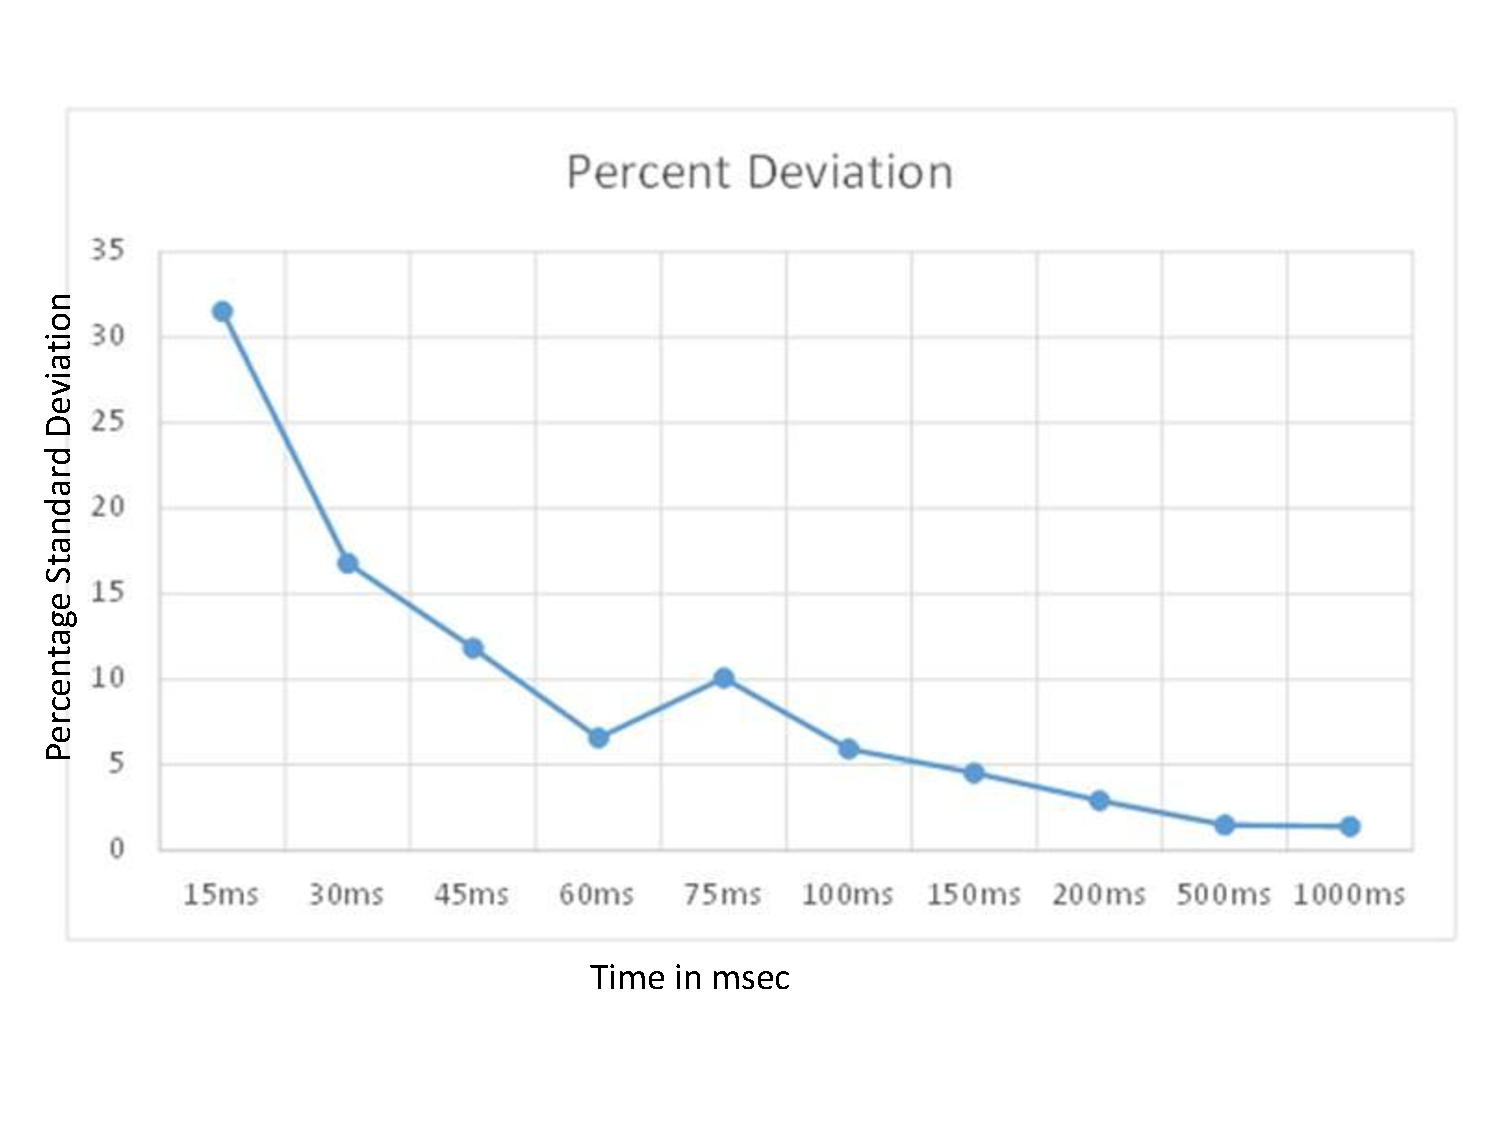
\includegraphics[width=\columnwidth, trim=60pt 20mm 0pt 8mm]{figures/variation}
\caption{Impact of $T$ on variance in $SR$}
\label{variation}
\vspace{-3mm}
\end{figure}

{\bf Discussion:} A value of $T$ between 60 - 100ms reduces standard deviation
of $SR$ to $5\%$.  Larger $T$ will lead to further reduction, but decrease is
small.

\subsection{Bandwidth Ramp Up and Ramp Down}
{\bf Question:} A VM may have to wait for up to 4 time intervals to reach its
minimum guaranteed bandwidth. Also, we wait for up to \fixme{1 second} before we
reclaim bandwidth from a VM that is not fully using the allocated bandwidth. Are
these time intervals appropriate?

{\bf Motivation:}  While the allocated bandwidth to VM ramps up to the minimum
guaranteed bandwidth in 4 intervals, the VM may not be able to ramp up as
quickly, due to limitations of the TCP congestion control. Furthermore, waiting
for \fixme {1 second} before reclaiming the bandwidth may lead to
under-utilization of the link.

{\bf Experiment:}  One of the test machines hosts 4 VMs with the following
minimum bandwidth guarantees: VM1: 100Mbps (relative weight = 1), VM2: 100Mbps
(relative weight = 1), VM3: 1Gbps (relative weight: 10), VM4: 3Gbps (relative
weight: 30) Each of the VMs sends traffic to the other machine ("client
machine") over the shared 10G external physical NIC.  Unless otherwise noted,
each VM is always backlogged and tries to send data as fast as it can.

Figure~\ref{fairsharing}  shows the transmit bandwidth for each VM, and the
total transmit bandwidth in several phases. 

\begin{figure}[h]
\centering
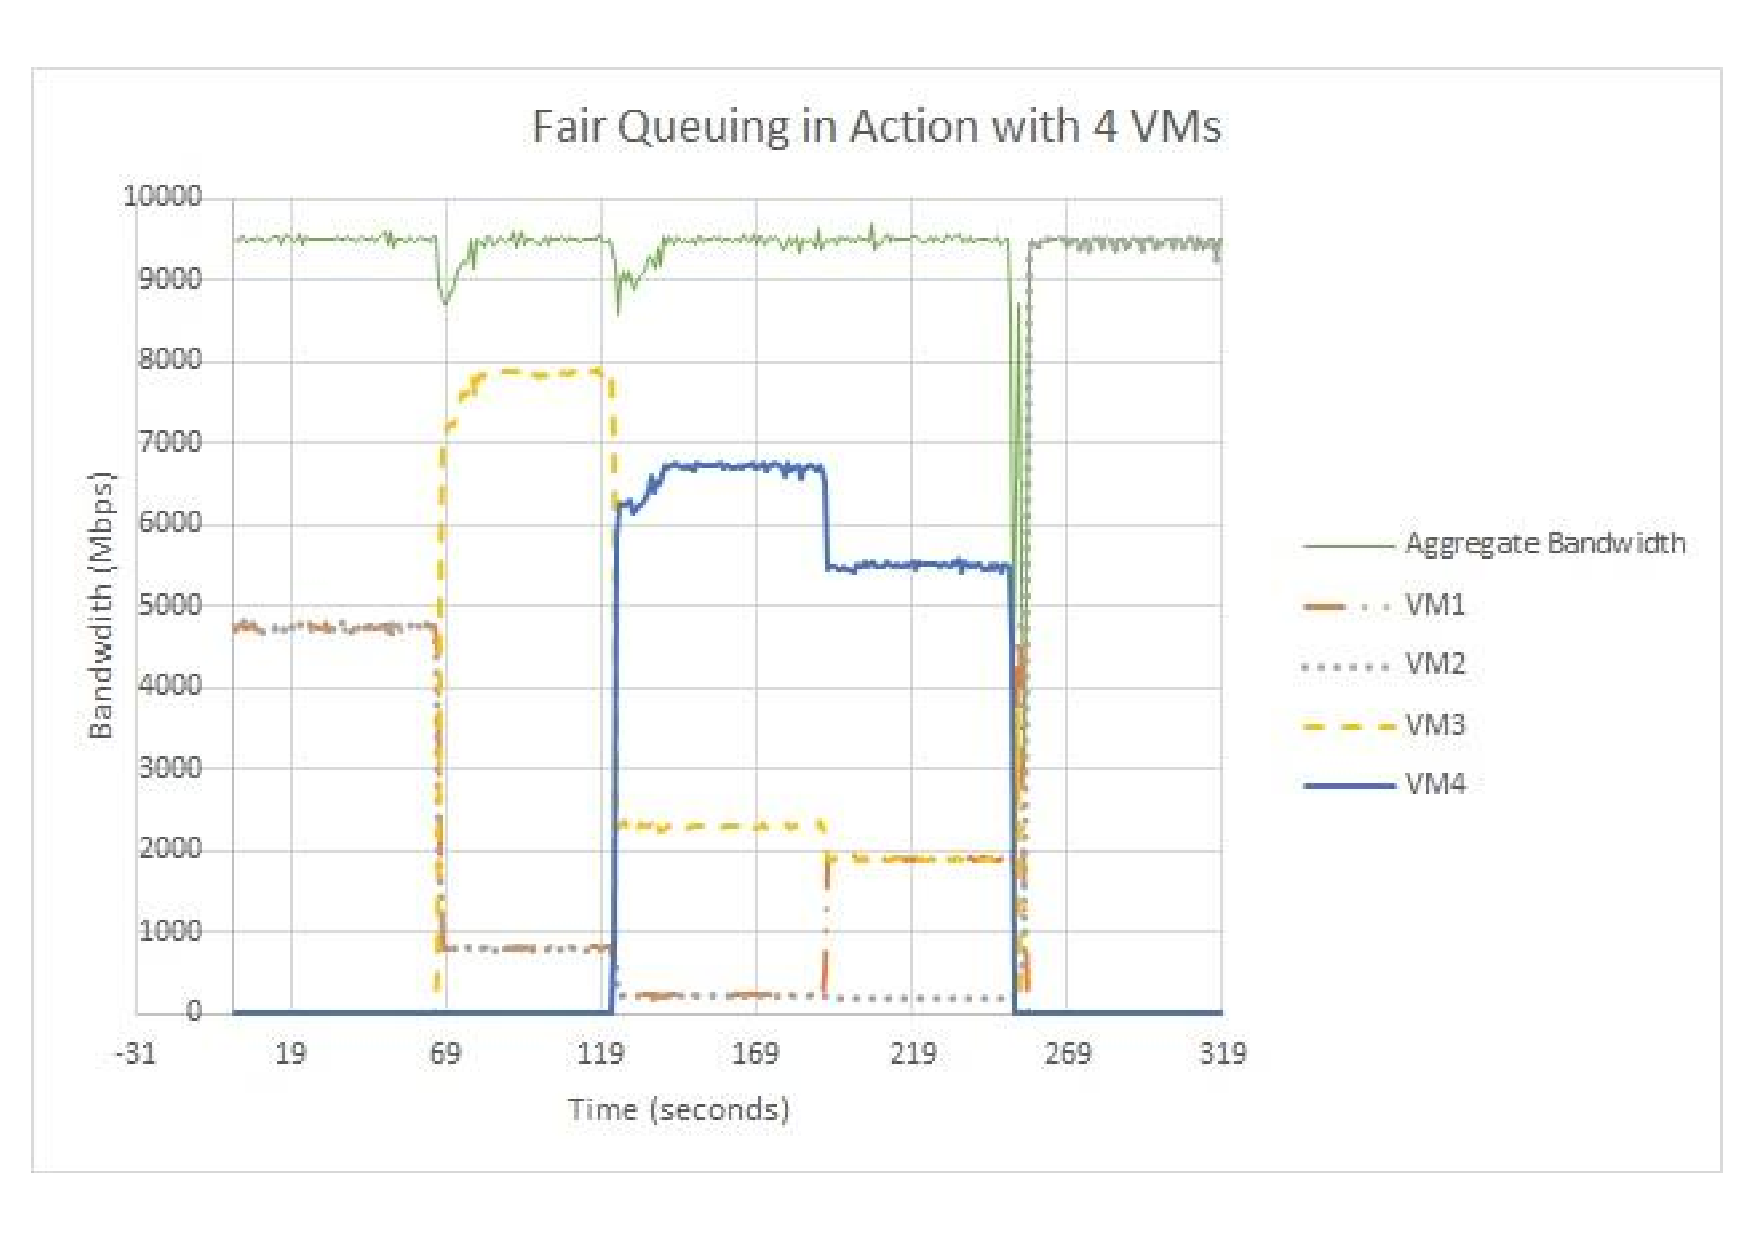
\includegraphics[width=\columnwidth,trim=60pt 20mm 0pt 8mm]{figures/fairsharing}
\caption{Ramp up and ramp down test}
\label{fairsharing}
\vspace{-3mm}
\end{figure}

{\bf Phase 1:}  At time 0, only VM1 and VM2 are active. As expected, they share
the bandwidth equally, with each getting about 5Gbps.

{\bf Phase 2:} At time \fixme{XXX}, VM3 starts transmitting. MBFQ quickly
throttles VM1 and VM2 to 833Mbps each, while VM3 is allowed to use 8.33Gbps. 

{\bf  Phase 3:} At time \fixme{xxx}, VM4 starts transmitting. The four VMs now
get their weighted fair share: VM1 and VM2 get 238Mbps, VM3
gets 2.38Gbps and VM4 gets 7.14Gbps. 

{\bf  Phase 4:} At time \fixme{XXX}, We change the min bandwidth guarantee of VM1 from 100Mbps to
1Gbps. We see that MBFQ allocation quickly converges to the expected rate of
\fixme{XXX}.

{\bf Phase 5:} At time \fixme{XXX}, VM3 stops sending. The new rate allocation is
\fixme{XXX}.

{\bf Phase 6:} At time \fixme{XXX}, VM1, VM3, and VM4 stop sending. VM2 quickly
ramps up to consume the full link bandwidth.

{\bf Discussion:} We see that while MBFQ generally performs well, there are dips
in link utilization at times \fixme{XXX}. The dips at the beginning of phases 3
and 4 are due to our desire to allow a customer to quickly attain minimum
guaranteed bandwidth. As VM3 and VM4 are ramping up, the algorithm detects that
the VMs requests for additional bandwidth in several consecutive iterations.
Therefore, in order to quickly provide the VMs their subscribed bandwidth, after
4 consecutive iterations of additional bandwidth requests, the algorithm
allocates the full fair share of bandwidth to the VM. \fixme{However, even after
    the bandwidth is allocated, it takes the VMs some time to consume it, due to
TCP artifacts.} Thus, the dip represents a trade-off between how fast the
algorithm should grant a VM its fair share versus how cautious it should be in
allocating the VM bandwidth that it might not be ready to consume (and thus risk
being non-work conserving). A more extreme dip is seen at the
beginning of phase 6, we shall discuss that later.

\subsection{Can we ramp up any faster?}

{\bf Question:}  Is the ramp up delay shown in Figure~\ref{fairsharing} for VM 4
at 69 seconds caused by our algorithm or it due to the VM itself (e.g., its TCP
behavior)?

{\bf Motivation:} The previous experiment suggests the algorithm may be too slow
in allocating bandwidth to a newly active VM.  

{\bf Experiment:} We measure bandwidth ramp up in two scenarios.  First, we
measure a  ``standalone'' scenario VM3 is the only VM transmitting (i.e. the link
was idle before VM3 started sending).  Second, we measure a  ``sharing'' scenario
in which the link was fully utilized before VM3 started sending. When VM3 starts
sending, MBFQ performs bandwidth allocation to give VM3 its fair share.

\begin{figure}[h]
\centering
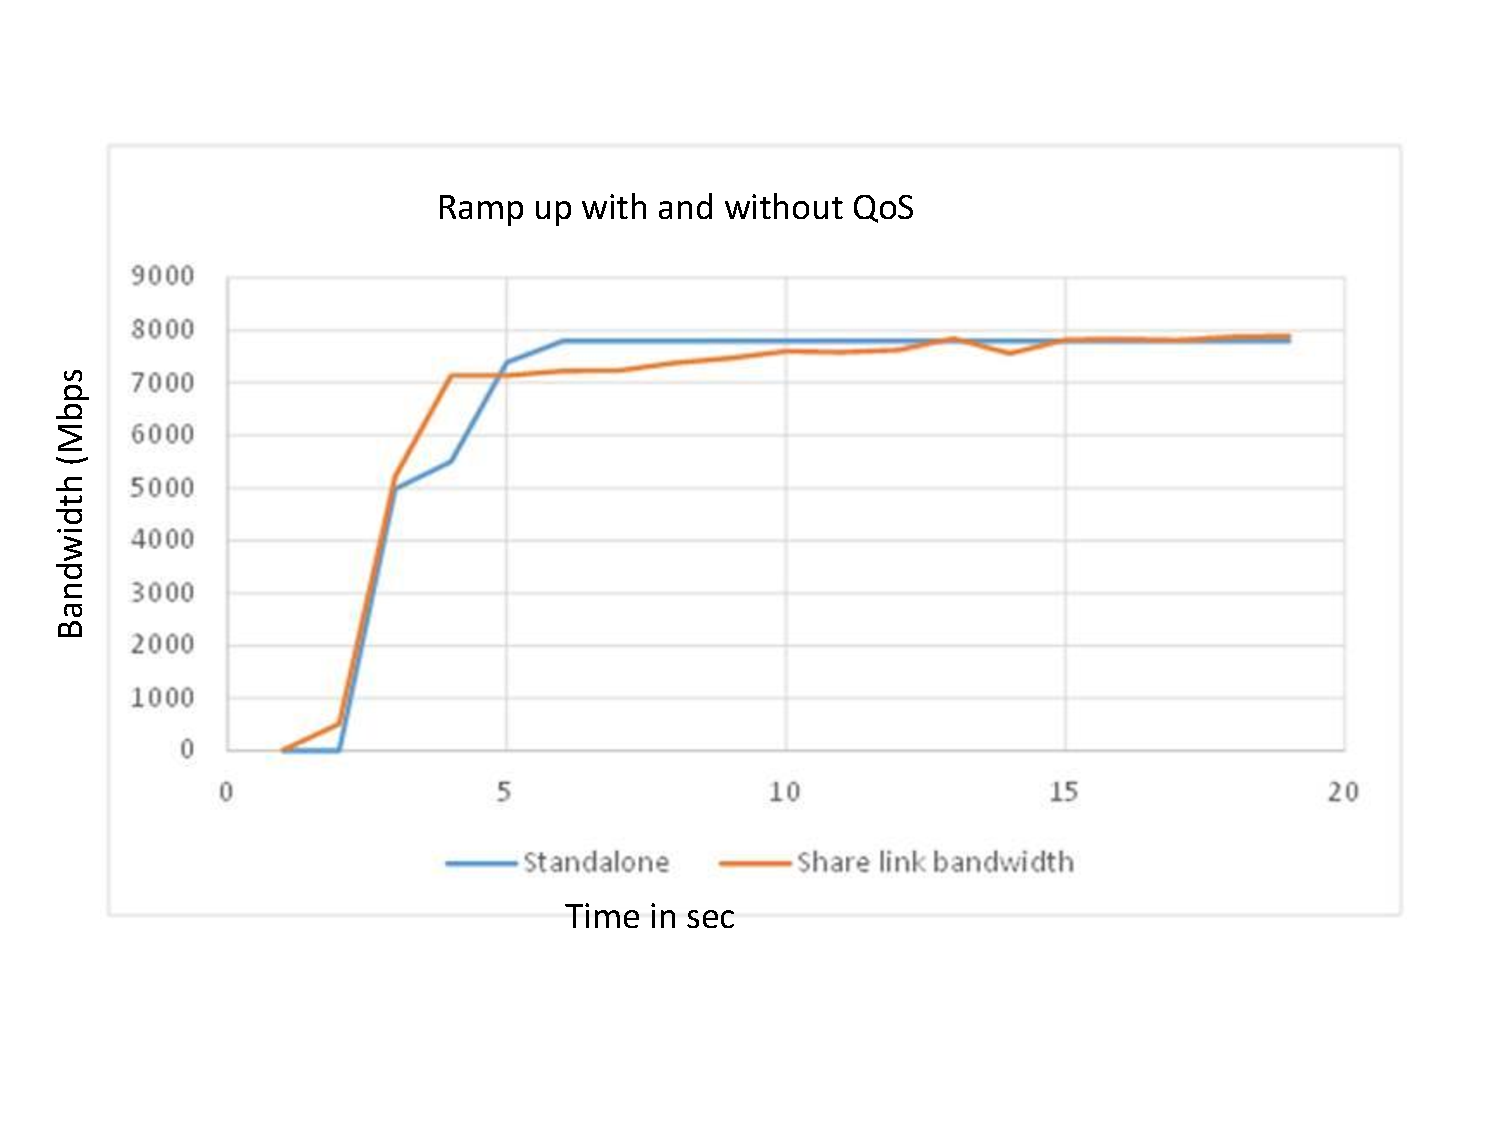
\includegraphics[width=\columnwidth,trim=60pt 40mm 0pt 8mm]{figures/rampupcomparison}
\caption{Comparing the ramp up speeds of TCP and MBFQ}
\label{rampupcomparison}
\vspace{-3mm}
\end{figure}

{\bf Discussion:} As seen in Figure~\ref{rampupcomparison}, it takes about the
same amount of time in both scenarios for VM3 to achieve most of its bandwidth
(up to 7Gbps). However, it takes an additional 15s for VM3 to reach its steady
state  in the "Share link bandwidth" scenario. However, in the sharing scenario,
the VM is transmitting on top of a NIC that is already fully utilized.
But in the standalone case, the VM is transmitting on top of an idle NIC. 

{\bf Conclusion:} It is probably not worthwhile 
to ramp up faster because TCP may not be able to fully utilize the extra
bandwidth quickly.

\subsection{How fast should we reclaim bandwidth?}
{\bf Question:}  The faster we reclaim bandwidth the
faster we redistribute it other needy VMs who can use it. How big should the
reclaim period $T$ be?

{\bf Motivation:} 
We see a large dip in the utilization at the beginning of Phase 6 in
Figure~\ref{fairsharing} when VM1, VM3, VM4 stop sending.  In addition to the
TCP ramp-up time of VM2, the dip is also partly due to another parameter in the
algorithm where we configure the algorithm to wait for \fixme{1s} before
reclaiming residual bandwidth  Unfortunately, this is a tradeoff.  The faster we
reclaim, the more likely the algorithm is to spuriously reclaim bandwidth from a
paid customer VM which has short term bursts.

{\bf Experiment:} : We have VM1, VM2, VM3 send CBR traffic. VM4 host a large
file that's being copied to a remote machine.  The file transfer application on
VM4 uses about 800Mbps, and the rest of the link bandwidth is distributed among
VM1, VM2, VM3.  We change the wait time parameter from No Wait (at every
macroshedular iteration, bandwidth is immediately reclaimed if the VM is
sending less than 85\% of its allocated rate) to 1000ms wait (bandwidth is not
reclaimed unless the VM has been sending less than 85\% of its allocated rate in
the last 1000ms)

\fixme{Combine these two figures, and rewrite}.
\begin{figure}[h]
\centering
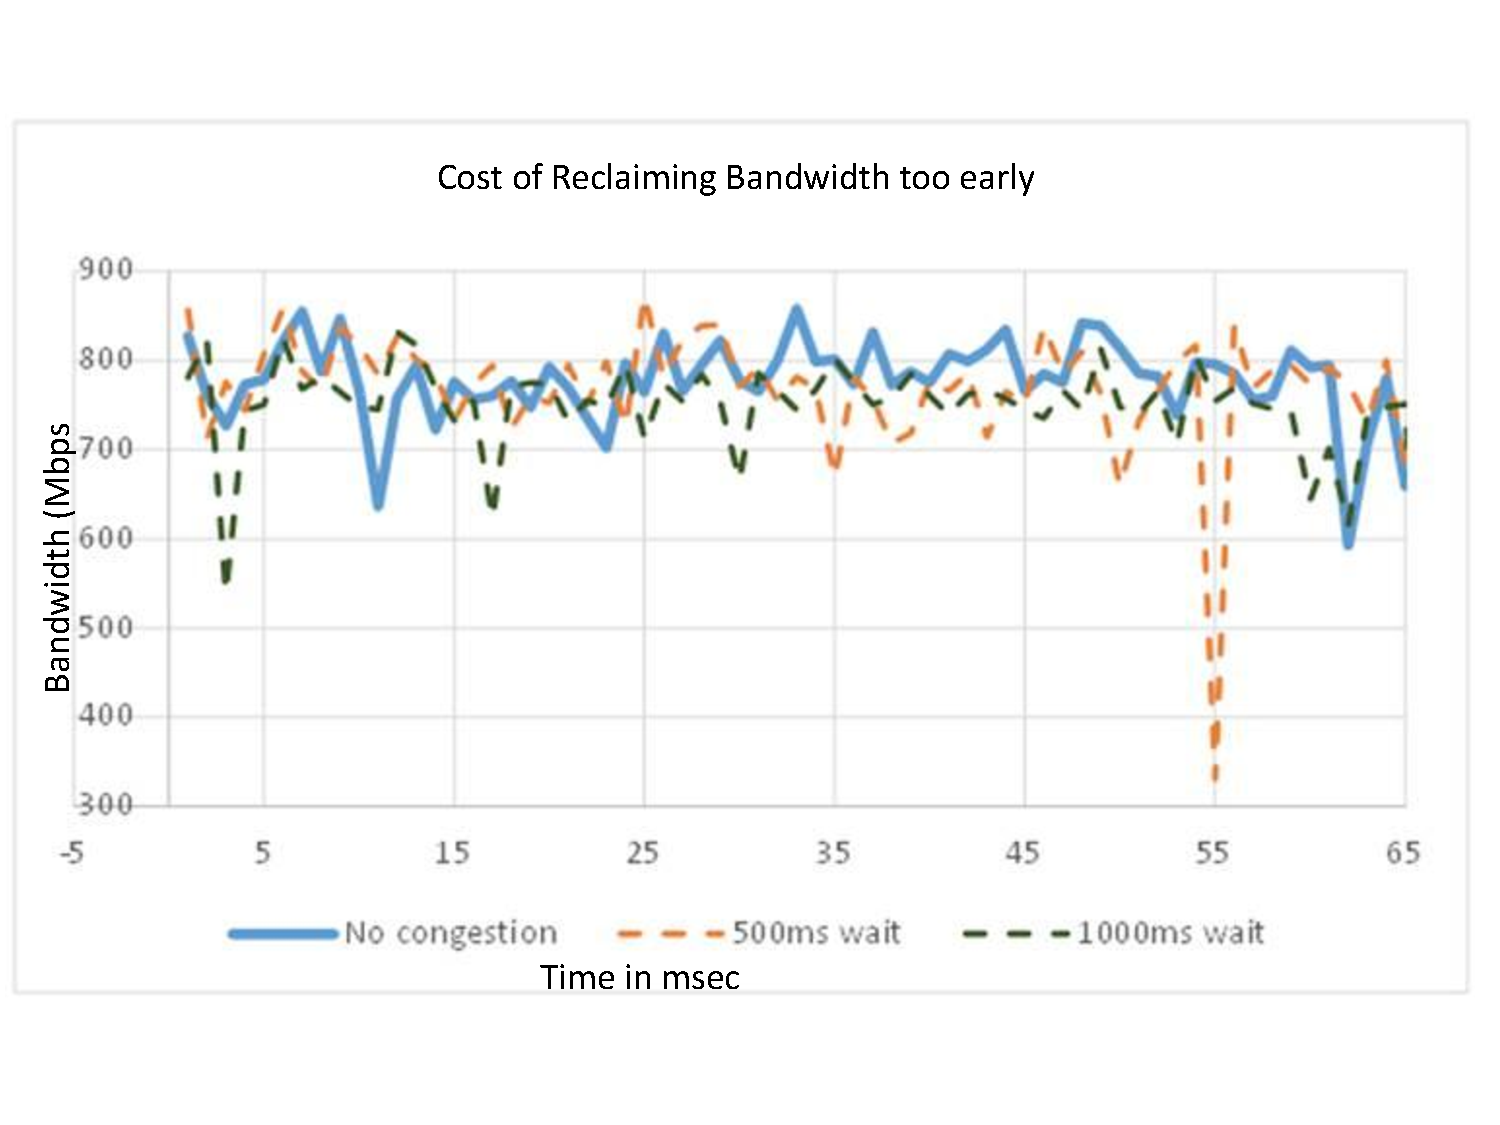
\includegraphics[width=\columnwidth,trim=60pt 20mm 0pt 8mm]{figures/rampdowntime1}
\caption{Bandwidth allocated to a bursty file transfer application with values of reclaim timer of 500 msec and 1000 msec}
\label{rampdowntime1}
\vspace{-3mm}
\end{figure}

Figure~\ref{rampdowntime1} shows that the bandwidth stays roughly the same with
MFQ and without MBFQ with a reclaim timer of 500 msec (in fact 1000 msec looks
even worse, but that could be an artifact).   On the other
hand,Figure~\ref{rampdowntime2} shows that with instantaneous reclaiming
(reclaim timer of 0) the bandwidth allocated to the VM is significantly affected
(by around 50\%) and its noticeable even at a reclaim timer of 200 msec.

\begin{figure}[h]
\centering
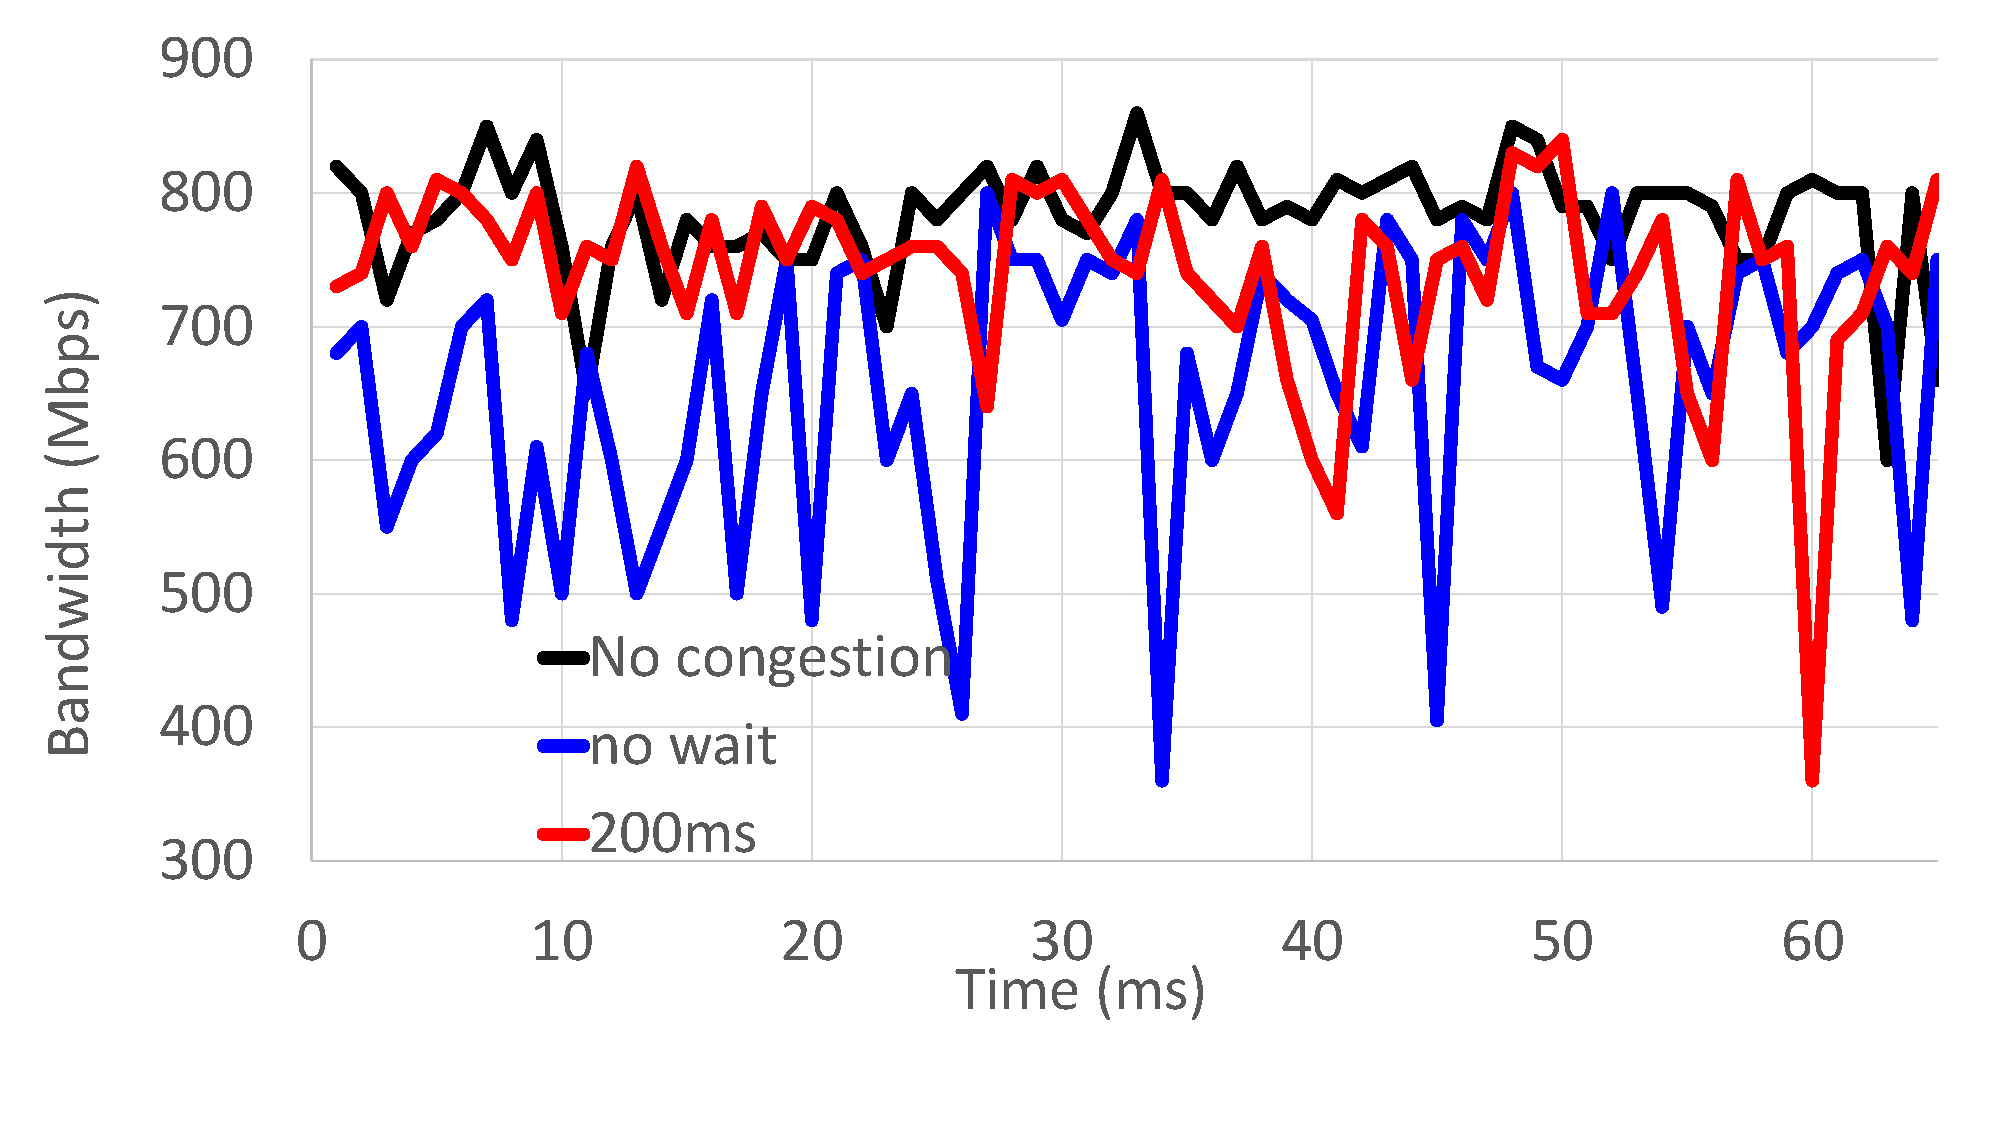
\includegraphics[width=\columnwidth,trim=60pt 20mm 0pt 8mm]{figures/rampdowntime2}
\caption{Bandwidth allocated to a bursty file transfer application with values of reclaim timer of 0 msec and 200 msec.  Notice the significant bandwidth loss due
to spurious reclamation}
\label{rampdowntime2}
\vspace{-3mm}
\end{figure}

{\bf Conclusion:}  A reclaim timer of around 500 msec seems like a good
compromise.  (Before our experimental evaluation, we had assumed that 1 sec
would be the right value). 
